%% Template file for all Software/Hardware modules

% Replace "Name of Module" with the name of this module
\chapter{Hardware Design Overview}

\section{Description}

The POW-R project is made of two main hardware components, the Server and the Satellites. The Server refers to the physical hardware from which the Display shall be served. It also acts as the data center for all Satellites associated to it, collecting data and administrating. The Satellites will talk over ZigBee specification to the one Zigbee module connected to the Server, and that one Zigbee module can talk to the Server over Universal Serial Bus (USB). Figure \ref{SystemOverview} shows the layout of the hardware system.


\begin{figure}
\centering
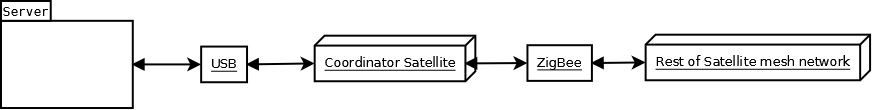
\includegraphics[scale=0.3]{Hardware/images/SystemOverview.png}
\caption{System Overview}
\label{SystemOverview}
\end{figure}

\section{The Server}
%% Template file for all Hardware modules

% Replace "Name of Module" with the name of this module
\subsection{PC Hardware}

\subsubsection{Mainboard}
The Server's main hardware component is the mainboard, a SYS9400-ECX Developer-Ready Reference Platform. 
It's a small form-factor, low-power machine with the following specs:

\begin{itemize}
	\item 1.6 GHz Intel Atom E6XX Series Processor
	\item 1 GB DDR2 RAM
	\item Roughly 6" by 4"
	\item Various connection interfaces:
	\begin{itemize}
		\item 2x SATA ports
		\item Header for Solid State Drive (SSD) power
		\item Ethernet port
		\item 5x USB 2.0 ports
		\item General Purpose Input/Output (GPIO) pin header
	\end{itemize}
\end{itemize}

\subsubsection{Potential Problems}
If for whatever reason using this mainboard falls through: 
It should be noted that the requirements for the Server hardware concern not just specifications, but interfaces as well.
In particular, this project requires at least Ethernet, 2 USB ports, a SATA port, and accessible GPIO pins.
\subsubsection{Storage}
The Server's mainboard is connected via SATA to a 40GB SSD.

\subsubsection{Power Supply}
An adapter rated for 12VDC @ 3A is used to connect the Server's board to mains electricity.

%% Template file for all Software/Hardware modules

\subsection{Add-Ons}
The Server provides for the computational needs of the POW-R project; 
More hardware shall be added before the utility needs of the project are met.

\subsubsection{IP Display}
The IP of the Server shall be displayed somewhere on it's casing. 
The user will enter this IP into their browser to access the Display.

This will be achieved by connecting an Arduino via USB to the Server, and housing it inside the Server's casing. 
The Arduino will be connected to an LCD display which will output the network IP of the Server. 
Figure \ref{ArduinoLCD} shows the interaction between Server and Arduino.

\begin{figure}
\centering
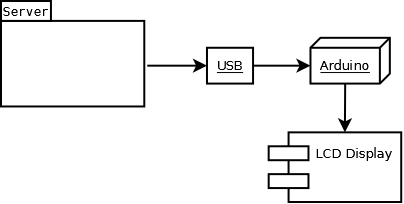
\includegraphics[scale=0.5]{Hardware/images/ArduinoLCD.png}
\caption{IP Display Diagram}
\label{ArduinoLCD}
\end{figure}

The IP of the system can be obtained via kernel module, and sent to the Arduino one byte at a time. 
This works well, since the Arduino connects over serial and thusly takes a byte at a time.

\subsection{GPIO Pins}
As mentioned above in the "PC Hardware" section, the mainboard is outfitted with a GPIO pin header. 
A Linux distribution will be used for the Server's operating system, which must support interaction with such pins. 

A folder can be found in the Linux kernel, at the location \filename{/sys/class/gpio} that helps with GPIO manipulation. 
To set up a single GPIO pin, one must type the following command into a terminal (as root):

\begin{lstlisting}
	$ echo N > /sys/class/gpio/export
	(where N must be a GPIO pin number)
\end{lstlisting}

When this command is issued, a directory is made inside the \filename{gpio} directory, named \filename{gpioN}, where N is the GPIO pin number you passed. 
Two files will be in that new directory, \filename{direction} and \filename{value}. 
\filename{direction} can only contain "in" or "out" with no leading characters, spaces, line breaks, etc.
\filename{value} can only contain "1" or "0" and can be read or written to at any time.
These files, \filename{direction} and \filename{value} are responsible for what kind of pin it is (input or output) and what the current value is (1 or 0), respectively.

NOTE: The pin number you must echo into \filename{/sys/class/gpio/export} is not necessarily the number of the actual pin on the board, but may refer to the pin of the bridge that connects the GPIO port to the motherboard.

The subsections below are buttons that the Server must have, and each of these buttons connects to a GPIO pin.


\subsubsection{Power Switch}
A standard rocker switch will be added to the case to provide the user with a way to turn the Server on and off. 
The style of the switch will clearly signify "On" or "Off".

\subsubsection{Factory Reset\repeatfootnote{opt}}
This button should intentionally be placed somewhere inconvenient: 
Sunken into the case far enough that you need a skinny rod (such as a paperclip) to push it, and in a spot
that chaotic forces (children, mean people, God's divine will) will not notice it.

\subsubsection{Connect to Satellite}
A button will be added to the Server that allows a user to add a Satellite easily.
When a user wants to add a Satellite to the network, the following series of events should take place, in order:

\begin{itemize}
	\item User plugs Satellite into wall outlet
	\item User presses "connect" button on Satellite
	\item User presses "connect" button on Server
	\item Satellite is now connected
\end{itemize}
	
\subsection{Server Hull}
The Server needs a protective casing, for several reasons. 
On the physical level, a durable casing will protect the hardware. 
The casing also serves to render unnecessary ports inaccessible to users. 
Lastly, the casing is important in the sense that the term "Server" currently only applies to the mainboard, 
and most people think of a legitimate Server as something physical, encased in a box, that's protected and hidden away, exactly as a Server should be.

As far as prototyping goes, the casing can be as simple as a folded piece of aluminum
with holes cut in it to fit the IP display, the buttons, and any ports that must be
exposed. As an end-game product, the casing would probably be a little less "junkyard."

\input{Hardware/Server-TalkToXbee}

\section{The Satellites}
The Satellites are made up of two sets of hardware: Instruments for measuring and radios for communicating. The end product shall have casing around it, NEMA 5-15 sockets on one side, and prongs for a NEMA 5-15 male end on the other. However, it should be noted that prototyping will most likely involve all of the hardware being spread out on breadboards.
%% Template file for all Software/Hardware modules

% Replace "Name of Module" with the name of this module
\subsection{Measurement Hardware}
Current and voltage running through the mains outlet to the Satellite's associated device must be measured and sent to the Server. 

%% Template file for all Software/Hardware modules

\subsection{Communications Hardware}

% Describe hardware setup for our
% XBee modules

For the communication between the Server and the Satellites,
we will be using the Xbee Series 2 Radio Modules.

\subsubsection{XBee Series 2 Radio Modules}

% Might want to mention we want series 2 for
% Zigbee, but ZigBee has it's own module since
% it's a fairly large part of this design

\subsubsection{Interface Board}

% This section is a little vague at the moment.
% Currently we're using Digi Interface Boards,
% but we may need to move to an Arduino if these
% boards lack an A/D converter pin. Haven't
% looked into it yet. In either case, whatever
% interface board we use will connect the
% measuring circuit to the radio. Might
% need diagram for this.

%% Template file for all Software/Hardware modules

\subsection{ZigBee Standard}
ZigBee is a standard that uses 802.15.4 wireless protocol as it's foundation. It's 
particularly useful for setting up ad-hoc mesh networks. Much like how any Bluetooth
devices can talk to each other, any ZigBee devices nearby can talk to each other (so 
long as they have the proper permissions).

\subsubsection{Why ZigBee?}
The advantage of using ZigBee is that it lines up with the requirements of the POW-R
project. It's a specification targeted for low-power, low-data applications that need
to be secure. 

Another advantage of using ZigBee is that XBee radios, which also fit the requirements
of the POW-R project, are ZigBee-compliant, so the forming of a mesh network can happen
quickly and easily.

\subsubsection{Device Types}
The nodes of a ZigBee network are obviously ZigBee devices, but from the network's
perspective, there are three distinct types of ZigBee device:

\begin{itemize}
	\item Coordinator
	\item Router
	\item End Device
\end{itemize}

The coordinator runs the network, keeps it healthy, makes sure everybody is talking when
they should be, and overall, just maintains the Mesh. It is also the device that is 
typically plugged into a computer via USB or some other serial interface, meaning
that this is the node you want to send data to. There cannot be a ZigBee network
without exactly one coordinator.

Routers are fully functional ZigBee modules, capable of taking care of themselves and
routing messages across the Mesh. Routers are capable of being "parent" devices.

End devices are low-power ZigBee devices that don't do any routing. They can only talk
to one other device, which is referred to as it's "parent" device. A router or a coordinator
may be a parent device, but not another end device.

In the POW-R project, the coordinator will be attached to the Server so that it may
also act as a data bridge between the Server and the Satellites. The rest of the 
Satellites are routers; There will be no end devices in the POW-R's mesh network.


\subsubsection{Network Topology}
Zigbee supports four network topologies, shown in Figure \ref{NetTopo}. A ZigBee network
is defined by two rules:

\begin{itemize}
	\item A ZigBee network must have two or more ZigBee devices
	\item One of those devices \emph{must} be a coordinator
\end{itemize}

As mentioned before, the POW-R project will use the Mesh configuration, but without end 
devices. This means that the Mesh will consist entirely of routers and one coordinator.

\begin{figure}
\centering
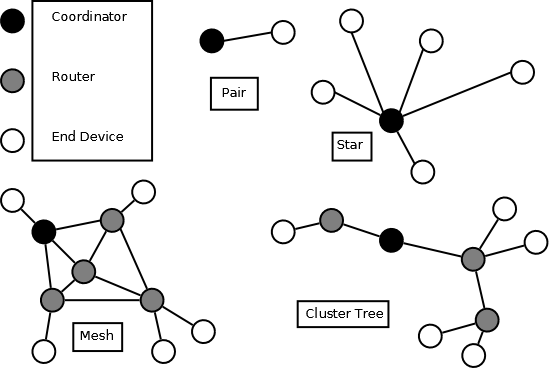
\includegraphics[scale=0.3]{Hardware/images/ZigBeeNetworkTypes.png}
\caption{ZigBee Network Topologies}
\label{NetTopo}
\end{figure}